\documentclass[11pt]{article}
\usepackage[legalpaper, portrait, margin=2cm]{geometry}
\usepackage{graphicx} %package for customizing pictures
\usepackage{wrapfig}
\usepackage{parskip}

\title{Lift Solutions}
\date{25/09/2023}
\author{Felix}
 

\begin{document}
\maketitle
\textbf{When} choosing our solution for the lifting of the fork it is important to specify the mast type
before hand or decide on designing a modular solution, where different mast´s can be mounted 
depending on the request of the customers. 

\begin{wrapfigure}{r}{0.5\textwidth}
    \begin{center}
        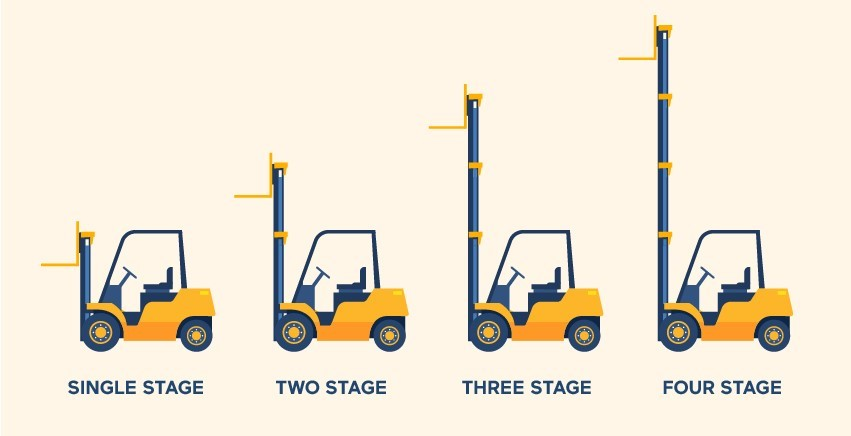
\includegraphics[width=0.40\textwidth]{../image/types-of-forklift-masts-1.jpg}
        \caption{Stages}
    \end{center}
\end{wrapfigure}
Those different mast types are called Simplex, Duplex, Triplex and Quadriplex which stand for the stage of
the mast assembly and in essence for the maximum height it can operate at.

For each stage after the Simplex the freelift is also of interest, as states at which point the mast 
will extend. Having full freelift allows the forklift to lift the fork until the top off a Simplex stage
without extending the mast, which makes the forklift useable in areas where not much overhead clearence is given,
for example when emptying a truck. 

\section{Real lifting systems}
Taking a closer look at the forklifts on the market, each lifting system is working with hydraulics. 
Reasons for this are:
\begin{enumerate}
    \item Ability to switch forks easily(clamping, rotating, extra long and changing width)
    \item Safety(Forks will never lower without permission) and no moving parts 
    \item Easy to maintenance 
    \item high power output
    \item precise control
\end{enumerate}
For lifting a hydraulic piston pushes a roller bearing up with a chain connected to an anchor on one side, rolling over 
it and connected with the fork on the other side. This creates a 2to1 lifting ratio where, 1meter lifted piston lifts the 
fork up 2meters.
\section{Lifting solutions}
Because of the high cost, low weight of load we will carry and not having the focus on a acurate downscalled 
forklift we won´t be able to use a hydraulic system for lifting.
Using a roller-chain should be considered in each solution for better load distribution and less movement need due to the 2to1
ratio.
Options can be:
\begin{enumerate}
    \item Linear Actuator(Bought)
    \item Linear Actuator(own design)(threaded rod)
    \item string+bearing 
    \item rack gear and pinion
    \item //any combination out of those for higher stages
\end{enumerate}
As our focus in this project lays on sensors and autonomous driving a Simplex stage 1 forklift will be enough of a mechanical 
task and could be upgraded if there is time to fill. 
Solutions could look like:
\begin{center}
    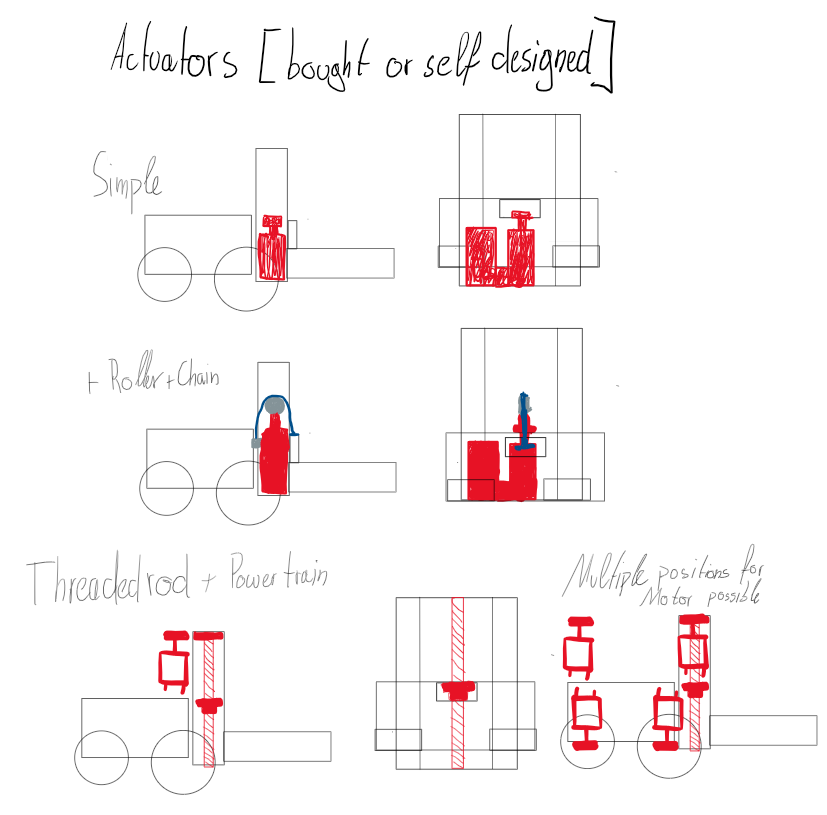
\includegraphics[width=0.9\textwidth]{../image/Liftsolutions1.png}
    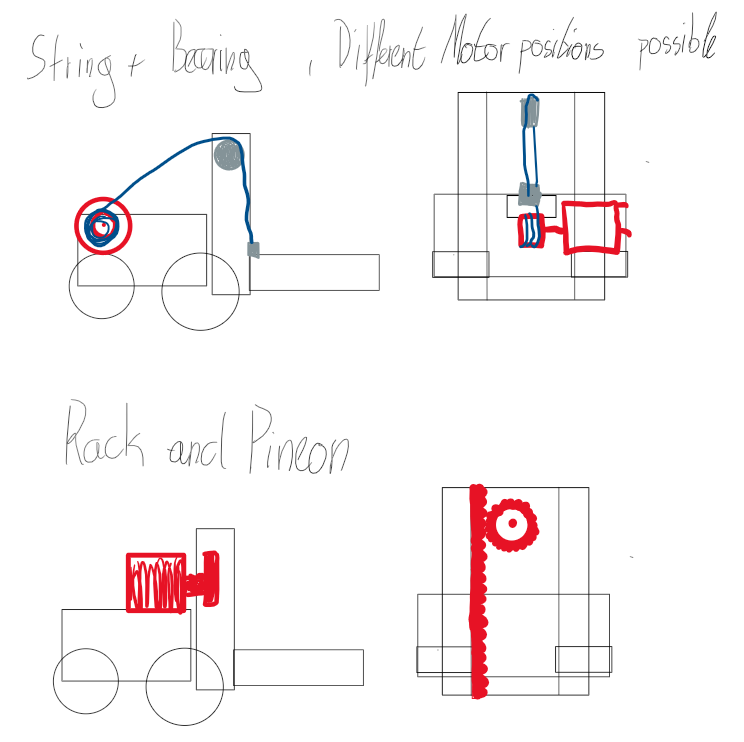
\includegraphics[width=0.9\textwidth]{../image/Liftsolutions2.png}
\end{center}
\section{Lifting Calculations}
To add a first value of safety the choosen system should be able to lift at least 30\% (to be defined by a standard later) more than the maximum weight
specification of our forklift. In this way we account for variances and fatique of the components we are working 
with.
We want to lift 4 beer cans per pallet and two pallets stacked which gives:
\[ 4*0.333*2*1.3=3.46kg\]
Including weight of pallets and fork into the 30\% and rounding up would give a plausible 3.5 kg actual lifting force or
\(3.5*9.81=34.5N\) which our lifting solution should be able to to provide.


\end{document}